\chapter{Desarrollo del proyecto}

\section{Extracción y recoleccion de datos}

\subsection{Introducción}

En el siguiente apartado se expone la metodología de obtención de los datos de entrenamiento.

Las distintas versiones de MoViNets están entrenadas sobre Kinetics 600 (REFERENCIA: \href{https://www.deepmind.com/open-source/kinetics}{KINETICS} ), por lo que para reentrenar el modelo necesitamos clips (videos) que representen los movimientos que se quieren predecir.

Si bien no existe un conjunto de datos similar aplicado específicamente a movimientos de crossfit, muchos atletas suben videos a youtube de realizando distintas pruebas y ejercicios. Partiendo de estos videos, se pueden extraer los distintos \textit{clips} (trozos) que representen los movimientos, con los que reentrenar el modelo.

Todos los videos descargados pertenecen a la primera etapa de los Crossfit Games de 2020 (REFERENCIA: \href{https://en.wikipedia.org/wiki/2020_CrossFit_Games}{CFGAMES2020}). Este año fue algo atípico debido a la pandemia. La competición se distinguió en dos etapas, una primera en formato online, y la final a la que solo pudieron acceder 5 hombres y 5 mujeres. Los videos correspondientes a la primera etapa están todos subidos a YouTube, donde todos los atletas están grabados de forma individual y con la cámara estática, lo que reduce enormemente el ruido de los datos.


\subsection{Proceso de extracción}

Para seleccionar la muestra de videos, se ha partido de 5 \textit{wods} (PONER NOTA AL PIE CON LA DEFINICIÓN) que en total dan pie a 9 movimientos (NOTA AL PIE, REFERENCIA A LABELS).

De cada \textit{wod} se han seleccionado 20 videos (10 de hombres y 10 de mujeres), de los cuales se han etiquetado 15 repeticiones de cada movimiento presente. Esto nos deja con una muestra de alrededor de 300 repeticiones por movimiento, 2700 clips.

Para descargar los videos se ha utilizado \href{https://github.com/yt-dlp/yt-dlp}{\texttt{yt-dlp}}, todos con la misma resolución (480x854p) en formato mp4. (INSERTAR NOTA AL PIE CON SCRIPT PARA LA DESCARGA, FALTA CREAR REPO A PARTE PARA LOS SCRIPTS)

El etiquetado de los videos se ha hecho con \href{https://supervise.ly/}{\textit{Supervisely}} \footnote{Tras probar otras alternativas como \href{https://labelstud.io/}{\textit{LabelStudio}}, \textit{Supervisely} facilita enormemente seleccionar rangos de frames por medio de atajos del teclado}.
Una vez se ha etiquetado un video, \textit{Supervisely} genera un \texttt{json} con las anotaciones correspondientes al movimiento y los frames en los que se produce.

Para obtener cada uno de los clips se ha utilizado (INSERTAR REFERENCIA A ffmpeg-split.py MIO)\footnote{Este script es una adaptación de \href{https://github.com/c0decracker/video-splitter}{\texttt{ffmpeg-split.py}}}. Las anotaciones se tranforman a un formato que \texttt{ffmpeg-split.py} pueda utilizar por medio de (INSERTAR REFERENCIA A \texttt{manifester.py}).

La figura \ref{data_extraction_process} resume el proceso para la obtención de los datos. (REFERENCIA A REPO Y DISTINTOS SCRIPTS)


\begin{figure}[H]
    \centering
		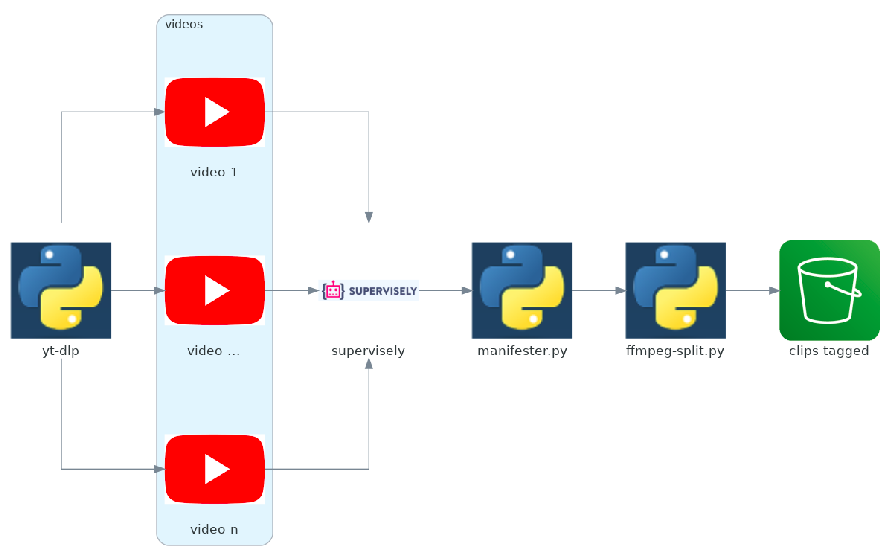
\includegraphics[height=10cm, width=12cm]{figs/data_extraction_process_.png}
\caption{Proceso de extración de datos}\label{data_extraction_process}
\end{figure}

\subsection{Datos obtenidos}

Meter tablas resumen de frames y segundos de los videos.


\section{Experimentación con deep learning}

texto

\subsection{Introducción}

texto

\subsection{Preprocesado de los datos}

(ESCRIBIR LA ELECCIÓN DE TENSORFLOW PARA EL DESARROLLO DEL MODELO)

De cara a construir la pipeline para el entrenamiento del modelo, se ha utilizado la API de \href{https://www.tensorflow.org/api_docs/python/tf/data/Dataset}{\texttt{tf.data.Dataset}} ya que permite la ingesta de un conjunto potencialmente grande de datos, así como el procesamiento de los mismos.

La forma más eficiente (BUSCAR REFERENCIA) de leer los videos en el \texttt{Dataset} es escribirlos como \href{https://www.tensorflow.org/api_docs/python/tf/data/TFRecordDataset}{\texttt{tf.data.TFRecordDataset}}, 
\texttt{tf.data.TFRecordDataset}
(REVISAR PARA QUE SALGA LA REFERENCIA)
para lo cuál se deben transformar los videos en formato mp4 a \texttt{tfrecords}. (INSERTAR REFERENCIA A movinets\_helper/writer.py, Y LOS DISTINTOS EJEMPLOS)

Al introducir los videos, se cambia el tamaño para igualarlo al utilizado en el entrenamiento original, 224x224p, y se escalan los valores para que se encuentren en el rango $[0, 1]$.

Para homogeneizar los datos de entrada se ha decidido fijar al número de frames para todos los videos a 10 ($\bar{f}=10$)(BUSCAR REFERENCIA A LOS DATOS UTILIZADOS EN EL PAPER ORIGINAL). Debido a que los vídeos en este conjunto de datos son más cortos que los utilizados en el caso de \textit{Kinetics 600}, se ha seleccionado el número de frames como $\bar{f} = \min_v f_{v}$, donde $f_v$ es el número de frames del vídeo $v$. El menor número de frames corresponde a uno de los vídeos de \textit{double-unders}. Para aquellos vídeos con un número de frames mayor que $\bar{f}$, se seleccionan $\bar{f}$ frames equiespaciados.


\subsection{Experimentos realizados y resultados}

El modelo se ha entrenado en \href{https://colab.research.google.com/?hl=es}{\textit{Google Colab}} con \textit{Tensorflow 2}. El modelo seleccionado ha sido MoViNets A2 Base\footnote{No ha sido posible hacer fine-tuning del modelo Stream debido a un error en los modelos guardados, ver \href{https://github.com/tensorflow/models/issues/10730}{issue 10730}.}, ya aunque sea necesario utilizar GPU para el fine-tuning, es el modelo más grande (con mejor capacidad predictiva) que permite hacer inferencia CON CPU en un tiempo razonable (BUSCAR REFERENCIA DE LOS AUTORES).

Los hiperparámetros del modelo son los mismos utilizados en el paper original (BUSCAR LOS DATOS EN EL PAPER ORIGINAL), con un tamaño de batch igual a 8\footnote{El tamaño del batch seleccionado es el mismo utilizado por los autores en el tutorial a modo de ejemplo sobre el dataset UCF101.}

La muestra se divide en un $80\%$ (2164 clips) para training, y un $20\%$ (541 clips) para test. (INSERTAR FIGURA DE LA DISTRIBUCIÓN DE LAS MUESTRAS AQUÍ).

El modelo se ha entrenado por 10 epochs, evaluando top 1 y top 5 accuracy, obteniendo un accuracy de 0.9995 y 1 en entrenamiento y test respectivamente.

El modelo base generaliza a un gran número de movimientos, incluyendo algunos movimientos similares (REVISAR LABELS DE SQUAT Y CLEAN QUE HAN METIDO), lo que puede facilitar seguir aprendiendo algunos de movimientos similares.

Por otro lado, los videos en este caso, aunque se han seleccionado de una muestra distinta de atletas, todos ellos son atletas de élite en su deporte, por lo que la ejecución de los movimientos son muy similares entre si, lo que facilita aprender a clasificar los mismos.

Los resultados del entrenamiento se pueden ver en de forma interactiva en \href{https://tensorboard.dev/experiment/UXyupsnMQ2S74vdul3vdbw/#scalars}{\textit{Tensorboard.dev}}

\subsection{Evaluación de los resultados}

A la hora de evaluar los resultados, empezamos analizando el heatmap de la matriz de confusión. Como se vio al analizar el accuracy en la muestra de validación, todos los movimientos se clasifican bien.

- INSERTAR heatmap matriz de confusión.

Con vistas a proporcionar un análisis más robusto, con un mayor número de movimientos o muestras de distintos atletas, puede ser útil la información que proporciona el heatmap REF. La construcción de este gráfico se hace de la siguiente forma. Partiendo de las probabilidades asignadas a cada vídeo en el período de test, se fija para cada movimiento (cada \textit{label}correcta) y se calculan las correlaciones. Se selecciona la correlación  (de Pearson) con el movimiento correctamente etiquetado, y se concatenan todos los vectores columna, de forma que obtenemos una matriz cuadrada. Estas correlaciones ayudan a ver cuáles son los movimientos que más se confunden entre si. Dado que las probabilidades deben sumar 1, aquellos movimientos con una correlación negativa más cercana a 1 son aquellos en los que se puede observar una mayor intercambio de probabilidades en la predicción.

(POR EJEMPLO, PONER ALGUNOS CASOS PARTICULARES DE LA TABLA Y CONTAR)

- heatmap matriz correlaciones (para ver con que otros movimientos se confunde).

Por último, se puede ver en la siguiente tabla las probabilidades medias y desviación estándar obtenidas para cada movimiento correctamente etiquetado. Esto nos permite ver cuáles son los movimientos que se predicen con una mayor confianza.

INSERTAR GRÁFICA DE LAS PROBABILIDADES POR CADA MOVIMIENTO EN EL ANEXO.

- tabla media/desv de las probabilidades para ordenar confianza en las predicciones.

\section{Cloud y despliegue de la aplicación}

En el siguiente apartado se presenta la aplicación para clasificar movimientos y su funcionamiento.

\subsection{Introducción}

texto

\subsection{Arquitectura cloud (diagrama)}

texto

\subsection{Resultado y funcionamiento (alguna imagen)}

texto
